\def\QRCODE{MASTER_mispa_TUT.IMG.ganip_matlabqrcode.png}
\def\QRPAGE{http://www.iptutorials.science/tree/master/MASTER_mispa/TUT.IMG.ganip/matlab}
\mcorrectionsection{Matlab correction}

\subsection{GAN}
In order to show the General Adaptive Neighborhood (GAN) of one image point, the following function is implemented.
Note that the function is given within the Classical Linear Image Processing (CLIP) framework, i.e. with the usual addition, subtraction and scalar multiplication. But the function could be generalized to other models such as the Logarithmic Image Processing (LIP).

\begin{matlab}
function RES = GAN(A,p,m)
% A is the original gray level image
% p is the image point coordinates
% m is the homogeneity tolerance
RES = zeros(size(A));
RES(p(2),p(1)) = 1;
s = A(p(2),p(1));
thresh = (A >= s-m) & (A <= s+m);
RES = imreconstruct(logical(RES),thresh,8);
\end{matlab}

\noindent In this way, we can visualize the GAN of any point of the 'Lena' image: 
\begin{matlab}
A=imread('lena256.bmp');
A=double(A);
p=[200,100];
mtol=[5,50,75];
GAN1=GAN(A,p,mtol(1));
GAN2=GAN(A,p,mtol(2));
GAN3=GAN(A,p,mtol(3));
figure
subplot(231);imshow(A,[]);title('original image')
subplot(232);imshow(A,[]);hold on;plot(p(1),p(2),'+r');title('seed point')
subplot(234);imshow(GAN1,[]);title('GAN / m=5')
subplot(235);imshow(GAN2,[]);title('GAN / m=50')
subplot(236);imshow(GAN3,[]);title('GAN / m=75')
\end{matlab}

\begin{figure}[htbp]
\centering
 \subfloat[Original image.]{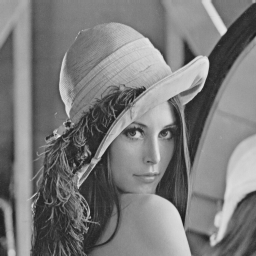
\includegraphics[height=.3\linewidth]{lena.png}}\hspace{1cm}
 \subfloat[Point location.]{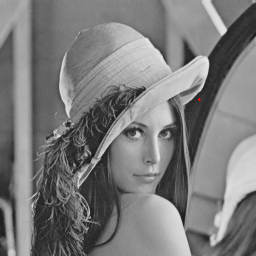
\includegraphics[height=.3\linewidth]{lenaPoint.png}}
 
 \subfloat[GAN (m=5).]{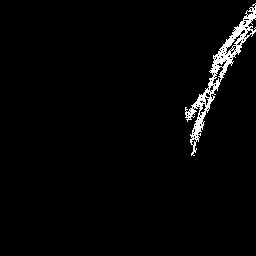
\includegraphics[height=.3\linewidth]{GAN1.png}}\hfill
  \subfloat[GAN (m=50).]{
\includegraphics[height=.3\linewidth]{GAN2.png}}\hfill
   \subfloat[GAN (m=75).]{
\includegraphics[height=.3\linewidth]{GAN3.png}}
 \caption{GAN of a specific point of the 'Lena' image using different homogeneity tolerances $m$ within the CLIP framework.}
\end{figure}

\subsection{GAN Choquet filtering}
In order to compute the GAN mean filtering, the basic idea is to make a loop on the image points, compute the GAN of the current point and then calculate the mean intensity of the points within the GAN. But this is time computing in the sense that two points with the same intensity can have exactly the same GAN (when one point is included in the GAN of the second point with same intensity). Therefore, a more effective way is to make a loop on the gray levels of the image.
The GAN mean filtering is then implemented as:

\begin{matlab}
function RES = GANmean(A,m)
% A: original image
% m: homogeneity tolerance
RES = zeros(size(A));
parfor s = 0:255
    thresh = (A >= s-m) & (A <= s+m);
    seed = (A == s);
    thresh = imreconstruct(seed,thresh,8);
    label = bwlabeln(thresh,8);
    nbLabel = max(label(:));
    for n = 1:nbLabel;
        currentLabel = (label == n);
        values = A(currentLabel);
        meanValue = mean(values);
        result = meanValue.*currentLabel.*seed;
        RES = RES + result;
    end
end
\end{matlab}

\noindent Looking at this function, for the first loop on the gray levels $s$, we detect the GANs of the pixels with gray level $s$. So 'thresh' contains all these connected components (GANs), where some points with identical gray levels $s$ can have the same GAN. 'label' enables the different GANs to be labeled. For the second loop on these GANs, we extract for each GAN its gray levels which are stored in 'values'. Afterwards, we take the mean value 'meanVaue'  that is stored as the resulting gray level for pixels inside the GAN with the same gray level $s$.

We can compare this GAN filtering with the classical one using a fixed operational window.

\begin{matlab}
h=ones(5,5)/25;
B=imfilter(A,h,'symmetric');
mtol=30;
C=GANmean(A,mtol);
figure
subplot(131);imshow(A,[]);title('original image')
subplot(132);imshow(B,[]);title('classical mean filtering')
subplot(133);imshow(C,[]);title('GAN mean filtering')
\end{matlab}

\begin{figure}[htbp]
\centering
 \subfloat[Original image.]{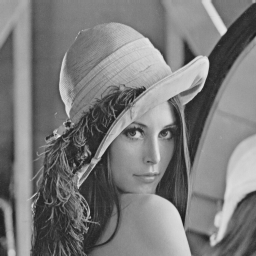
\includegraphics[height=.3\linewidth]{lena.png}}\hfill
 \subfloat[Classical filtering ($r=5$).]{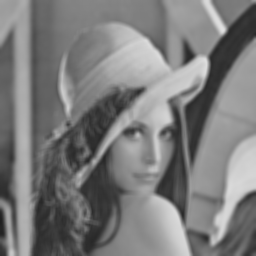
\includegraphics[height=.3\linewidth]{lena_classicalMean.png}}\hfill
  \subfloat[GAN filtering ($m=30$).]{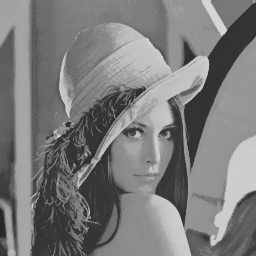
\includegraphics[height=.3\linewidth]{lena_adaptiveMean.png}}
 \caption{Classical ($r=5$) vs. GAN ($m=30$) mean filtering of the 'Lena' image.}
\end{figure}

\noindent You can see the blurring effect caused by the classical filtering, contrary to the adaptive GAN filtering where the transitions are much more preserved while smoothing the image. 

\subsubsection{GAN morphological filtering}
The followinh codes enable the GAN dilation and erosion to be computed. As previously mentioned, it is based on a loop on the gray levels and not on the image points. Note that the GANs ae computed on the criterion image (it is important for satisfying the good properties of opening and closing, such as idempotence).

\begin{matlab}
function RES = GANdilation(A,h,m)
% A: original image
% h: criterion image
% m: homogeneity tolerance
RES = zeros(size(A));
parfor s = 0:255
    thresh = (h >= s-m) & (h <= s+m);
    seed = (h == s);
    thresh = imreconstruct(seed,thresh,8);
    label = bwlabeln(thresh,8);
    nbLabel = max(label(:));
    for n = 1:nbLabel
        currentLabel = (label == n);
        values = A(currentLabel);
        values = sort(values);
        result = double(values(length(values)))*currentLabel;
        RES = max(RES,result);  
    end
end
\end{matlab}

\begin{matlab}
function RES = GANerosion(A,h,m)
% A: original image
% h: criterion image
% m: homogeneity tolerance
RES = 255*ones(size(A));
parfor s = 0:255
    thresh = (h >= s-m) & (h <= s+m);
    seed = (h == s);
    thresh = imreconstruct(seed,thresh,8);
    label = bwlabeln(thresh,8);
    nbLabel = max(label(:));
    for n = 1:nbLabel;
        currentLabel = (label == n);
        values = A(currentLabel);
        values = sort(values);
        result = double(values(1))*currentLabel+255*(~currentLabel);
        RES = min(RES,result);
    end
end
\end{matlab}

The following script shows the difference between classical and adaptive morphology.

\begin{matlab}
se=strel('disk',2);
Bdil=imdilate(A,se);
Bero=imerode(A,se);
mtol=30;
Cdil=GANdilation(A,mtol);
Cero=GANerosion(A,mtol);
figure
subplot(231);imshow(A,[]);title('original image')
subplot(232);imshow(Bdil,[]);title('classical dilation')
subplot(233);imshow(Bero,[]);title('classical erosion')
subplot(235);imshow(Cdil,[]);title('GAN dilation')
subplot(236);imshow(Cero,[]);title('GAN erosion')
\end{matlab}

\begin{figure}[htbp]
\centering
 \subfloat[Original image.]{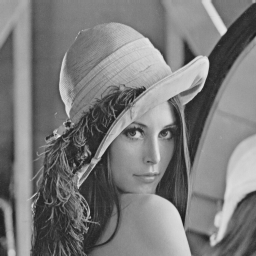
\includegraphics[height=.3\linewidth]{lena.png}}\hfill
 \subfloat[Classical erosion ($r=2$).]{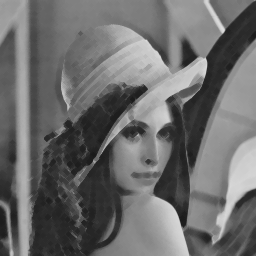
\includegraphics[height=.3\linewidth]{lena_classicalErosion.png}}\hfill
  \subfloat[Classical dilation ($r=2$).]{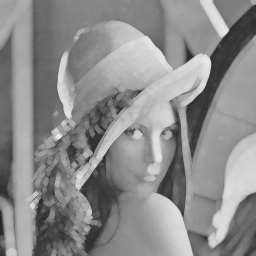
\includegraphics[height=.3\linewidth]{lena_classicalDilation.png}}
  
  \hspace{.3\linewidth}\hfill
  \subfloat[GAN erosion ($m=30$).]{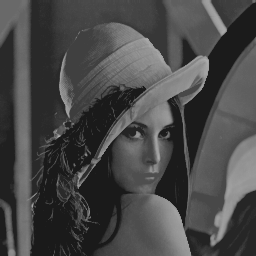
\includegraphics[height=.3\linewidth]{lena_GANErosion.png}}\hfill
    \subfloat[GAN dilation ($m=30$).]{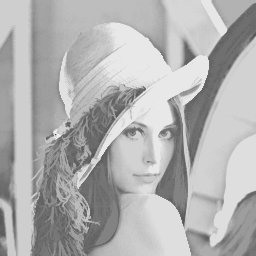
\includegraphics[height=.3\linewidth]{lena_GANDilation.png}}
 \caption{Classical ($r=2$) vs. GAN ($m=30$) morphological filtering of the 'Lena' image.}
\end{figure}

\noindent As previously mentioned with the Choquet filtering, you can see the blurring effect caused by the classical filtering, contrary to the adaptive GAN filtering where the transitions are much more preserved while smoothing the image.

Now, we can compute the GAN opening and closing as combined operators of dilation and erosion.

\begin{matlab}
function RES = GANopening(A,h,m)
% A: original image
% h: criterion image
% m: homogeneity tolerance
temp = GANerosion(A,h,m);
RES = GANdilation(temp,h,m);
\end{matlab}

\begin{matlab}
function RES = GANclosing(A,h,m)
% A: original image
% h: criterion image
% m: homogeneity tolerance
temp = GANdilation(A,h,m);
RES = GANerosion(temp,h,m);
\end{matlab}

It is very important to use the same criterion $h$ when combining these two operators of GAN dilation and erosion. It means that we compute the GANs at the beginning and therefater we use these same GANs for computing dilation and erosion. It enables the idempotence, extensivity/anti-extensivity of the GAN opening and GAN closing to be satisfied.

\begin{matlab}
Copen = GANopening(A,A,mtol);
Cclose = GANclosing(A,A,mtol);
figure
subplot(131);imshow(A,[]);title('original image')
subplot(132);imshow(Copen,[]);title('GAN opening')
subplot(133);imshow(Cclose,[]);title('GAN closing')
\end{matlab}

\noindent The result of such morphological filters is presented in Fig.\ref{fig:ganip:matlab:openingclosing}.

\begin{figure}[htbp]
\centering
 \subfloat[Original image.]{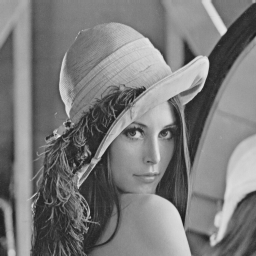
\includegraphics[height=.3\linewidth]{lena.png}}\hfill
  \subfloat[GAN opening ($m=30$).]{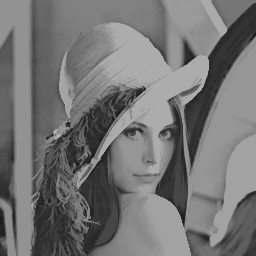
\includegraphics[height=.3\linewidth]{lena_GANOpening.png}}\hfill
    \subfloat[GAN closing ($m=30$).]{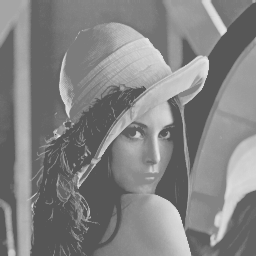
\includegraphics[height=.3\linewidth]{lena_GANClosing.png}}
 \caption{GAN ($m=30$) opening and closing of the 'Lena' image.}
 \label{fig:ganip:matlab:openingclosing}
\end{figure}

We can check some properties of these morphological filters such as extensivity/anti-extensivity and idempotence:

\begin{matlab}
Copen = GANopening(A,A,mtol);
Copen2 = GANopening(Copen,A,mtol);
Cclose = GANclosing(A,A,mtol);
Cclose2 = GANclosing2(Cclose,A,mtol);
% extensivity/anti-extensivity:
min(min(Copen<=A)))
min(min(Cclose>=A)))
% idempotence
min(min(Copen2==Copen)))
min(min(Cclose2==Cclose)))
\end{matlab}

\noindent The result is $1$ for all these Boolean tests.
